\documentclass[a4paper,10pt]{article} % {{{
\usepackage{listings,amssymb,amsmath,amsthm,graphicx,float,hyperref}

\hypersetup{
    colorlinks=false,
    pdfborder={0 0 0},
}
\newcommand{\tsup}[1]{\ensuremath{\sp{\text{#1}}}}

\author{Harm Dermois (5027963) \\ Joris Stork (6185320) \and
Lucas Swartsenburg (6174388) \\ Sander van Veen (6167969)}

\title{Cobots and Sun SPOTs}

% }}}

\begin{document}

\maketitle

\abstract{This project concludes our team's involvement in a January 2011
robotics course at the University of Amsterdam (UvA). The team consists of four
second-year UvA students enrolled for the BSc in Computer Science. The overall
aim of this project is to address the challenges inherent in programming a
microcontroller based mobile robot and handling communication between multiple,
different devices.}

\tableofcontents

\pagebreak

\section{Introduction} % {{{

Our team was given the task, firstly, of ``resuscitating'' the UvA's
Java-programmable ``Jobot'' robots, whose software development platform had
become defunct and inoperative. Our second task was to combine the Jobots'
mobility and sensing capabilities with the enhanced communications, sensing and
processing functionality of Sun SPOTs -- wireless sensor network devices from the
Sun Labs stable. In this way, we hoped to achieve a few things, namely to:

\begin{itemize}
    \item write, compile and load programs from scratch for a PIC based
    microcontroller board;
    \item create drivers for the servos and sensors connected to the board
    mentioned above;
    \item further explore the Sun SPOTs' sensing and communications
    characteristics through those devices' Java frameworks;
    \item build a data communication channel between the Sun SPOTs and the
    standard microcontrollers on the Jobots. Investigate if it is possible
    to transmit the data over an $I^2C$ bus;
    \item design an interface between our respective software implementations on
    the Jobot and on the Sun SPOTs;
    \item build a remote control system using the above interface;
    \item attempt some basic robot activities using our adapted, Sun SPOT
    controlled robot(s), such as: obstacle avoidance; reaching a goal;
    recognising a fellow robot; following a fellow robot, and so on, and;
    \item learn to work with embedded chips and low-level signal handling.
\end{itemize}

Strict time and resource limitations took precedence over any adherence
to pre-formulated goals and methods. That said, our project was successful,
and our team achieved a bonus on the way.

This report describes the principal materials at our disposal and our approach
to completing the given project tasks. Our results are described per challenge,
in chronological order of their occurrence. This approach reflects the
exploratory nature of the project, in which a string of unexpected obstacles
dictated the structure of our efforts over the past two weeks.

% }}}

\section{Materials} % {{{

Appendix

% Is it wise to store this section in the appendix or here?

% }}}

\section{Approach} % {{{

\subsection{Cobot} % {{{

% }}}

\subsection{Sun SPOTs} % {{{
\label{sec:sunspot}

The Sun SPOT is a vital part of our project. We use the Sun SPOT to control the
robots. Initially, it was our plan to have communication between the robots
through these Sun SPOTs. Also, the information from the Robot's sensors were to
be sent to the Sun SPOTs to be interpreted and handled accordingly.

% }}}

\subsection{Communication between the Sun SPOTs} % {{{
\label{subsec:comm}

The first order of business was getting the Sun SPOTs to communicate with each
other. To do this you need to use the function on the Sun SPOT to start
listening for information. It is almost always required to filter some of these
packages, because if there are other Sun SPOTs communicating with each other.
You need to be sure you are receiving the right packages. We haven't implemented
this, because we were working in a secluded area away from other sunspots which
might interfere with out Sun SPOTs, but this is easily implemented in the code
we made. In the final code we do filter out packages without valid commands.
This will avoid most of the unwanted traffic, but we can still get some messages
that were not intended for us.

We send some information in the form of tilting the Sun SPOT. This chosen to
figure out both how to send the information and to get to know how the
sensors(EDemoboard) of the Sun SPOT functioned. We wanted the communication
between to be both ways. So we had to use threads to get this working properly.
Without threads you will often get stuck because of desynchronization and would
be waiting on each other.

With the implementation of theses thread we finally managed to correctly send
the information between the two Sun SPOT. We built the foundations of the
communications between the two robots or as application as a remote control.
With this foundation it could be used to implement any sort of data transfer in
an orderly fashion and with the way we made the code it is very easy too expand
it for more difficult problems.

% }}}

\subsection{Bit-banging} % {{{
\label{subsec:bitbang}

%Bit-banging can be implemented at very low cost, and is used in, for example,
%embedded systems.

First we thought we could send the data between the Sun SPOT and the Cobot via
the $I^2C$ bus, but halfway through the project. It was found out this wasn't
possible, because of a technical issues. Namely the Sun SPOT can only handle a
voltage of 3V and the Cobot can only send signals of 5V. This is a big problem
if you want to communicate between the two without frying the Sun SPOT. Luckily
the Cobot can register voltages of 2V and higher so no modification had to be
made to get this to work.

This meant we had to use another method to get the information to the Cobot. The
solution that was given to us was the use of bit-banging. Bit-banging is a
technique for serial communications using software instead of dedicated
hardware. This means you got to send all the information bit by bit instead of
sending a full package of bytes in the form on any given data type. If you want
to use this method it is needed to have good control of how and when the
information is sent. This means you are responsible for all the timings and
synchronizations between the parties. The good thing about bit-banging is that
it is low cost. It gives you more control and the best thing is that it can be
used in every languages and can be used on every system that can communicate
with software, because it is so low level.

In our case we started by first sending information between two Sun SPOTs. We
wanted to implement big-banging without the use of a clock. So there's a
handshaking protocol need to get the two aligned. Here goes a picture of our
handshaking protocol so just a picture of when each line is high or low.

% }}}

\subsection{Bringing the pieces together} % {{{
\label{subsec:Bringing the pieces together}

Now that we have both the Cobot ready to drive and the bit-banging between the
Sun SPOTs. We can finally start putting the pieces together. Although we had all
the pieces, it was still hard to get them to work together properly.

% TODO: describe different Voltage of the devices, since that is the reason we
% couldn't use I^2C for data transfer between the Sun SPOT and the Cobot.

% We had some difficulties converting the implementation we had working on our Sun
% SPOT (in Java) to work on the Cobot (written in C). The problems were mostly
% because of the limitations of the compiler we had in for the Cobot.

Also, we initially used timers for the Sun SPOTs to send datagrams to each
other. We could not use this timers from the Java code, since those timers did
not guarantee that a bit is transmitted: there is no guarantee the timers of
both devices are working correctly. We went for a deterministic approach by
implementing a state machine. The basic idea is really simple (you could only
transition from one state into another), but you have to make sure acknowledge
bits are continuously sent to both sides. In figure ~\ref{fig:handshaking} is
shown how the transmission protocol for bit banging works, without using a
clock.

\begin{figure}[H]
\label{fig:handshaking}
\centering
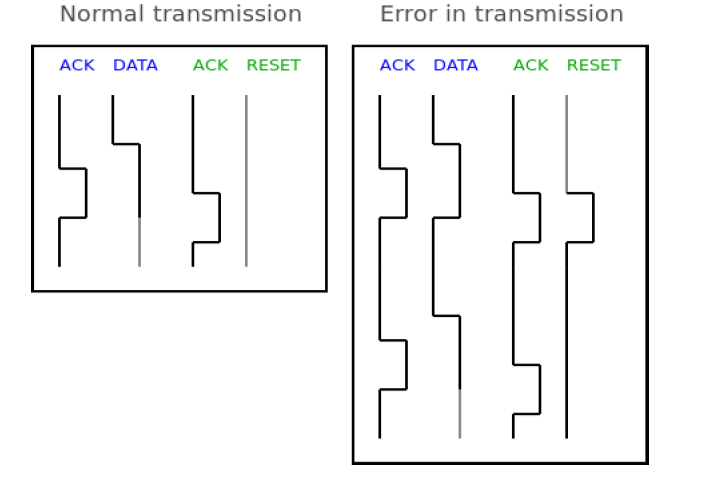
\includegraphics[width=11cm]{img/handshaking.png}
\caption{The left image is a bit diagram of a normal transmission and right is a
simplified example of an error occurred during the transmission. To send one bit
from a device (blue labelled lines; sender) to another device (green labelled
lines; receiver), first put your data pin on the value you want to send. Then
you put your ACK flag on. Now, the receiver knows the sender is ready to send a
bit.  When the receiver sees the sender's ACK flag, the receiver read the value
of the data pin and puts his acknowledge flag on. When the receiver set its ACK
flag, the sender knows the message bit is received. The sender lowers its
acknowledge flag, and the receiver will followed by lowering its own ACK flag as
well. When both ACK flags are down, the process starts all over again. There is
also a reset flag, which indicates a restart of the whole process is required.
The receiver will set its reset flag, when an invalid value is received.}
\end{figure}

% }}}

% }}}

\section{Implementation} % {{{
\label{sec:Implementation}

\subsection{Cobot implementation} % {{{
\label{sub:Cobot implementation}

% }}}

\subsection{Sun SPOT implementation} % {{{
\label{sub:Sun SPOT implementation}

For this project we used one Sunspot to determine the movement of the robot (by
measuring the tilt) and sending that information using a wireless connection to
the other Sun SPOT. The other Sun SPOT will receive the datagram sent and uses
bit banging to send the received movement to the Cobot. Both Sun SPOTs start up
a \texttt{BootloaderListenerService}, so that we can read the debug output at
real-time on our computer. This was very useful to debug the Java code. Both
Sunspots extend the \texttt{javax.microedition.midlet.MIDlet} class, so that all
the functions the Sun SPOT needs to operate are in the code.

\subsubsection{Measure tilt and send wireless datagrams.} % {{{

Two threads are used to enable measuring tilt while sending datagrams. It is
necessary to create two threads, because sending/receiving datagrams is a
blocking operation. If a single thread is used for both tasks, the tilt is not
measured until the sending/receiving process is done.
\\
\\
\noindent Thread 1: \textbf{Measuring the tilt and determine what the next Cobot's
movement is or if the Cobot should halt.}
\\
\\
This thread continuously measures the tilt of the Sunspot. After measuring the
tilt, the next movement of the Cobot is determined by checking if the Y tilt is
larger than the X direction and by measuring if the tilt of either the Y or the
X direction is larger than 25 degrees. When this is not the case, the Sunspot
will set the movement to ``stop'' (thus no movement). If this is the case and X
is larger than Y, the Sunspot will set the direction to left or right. If the
tilt is negative, the Sun SPOT will turn right and vice versa.  Pretty much the
same case if the tilt in the Y direction is larger than the tilt in the X
direction. After the movement of the Cobot is determined, the LEDs are set in
such way that it is clear what is measured.
\\
\\
\noindent Thread 2: \textbf{Sending a wireless package to the other Sunspot
containing the direction.}
\\
\\
This thread determines if the movement variable has been changed. If the
movement variable has changed, it will send a radiogram containing the
corresponding value of the movement to the other sunspot. Before this is
possible, a radio connection has to be established. The connection is made using
this function call: \texttt{Connector.open("radiogram://broadcast:37")}.

And a so called ``datagram'' has to be made. We write the integer that contains
the direction information to the datagram and this datagram is send to the other
Sunspot.

% }}}

\subsubsection{Receive movement and communicate with the Cobot} % {{{
TODO ...
\\
\\
\noindent Thread 1: \textbf{Receive the datagrams sent by the Sun SPOT.}
\\
\\
After the direction has been sent, the Sun SPOT sets the LEDs in a way that
it is clear what the received direction is. It will also start up the bit
banging process.

% }}}

\subsubsection{Sun SPOT / Cobot handshake} % {{{
\label{subsub:Sun SPOT / Cobot handshake}

Before the second Sun SPOT starts receiving, it first needs to get a handshake
from the Cobot. The handshake is given when the Sunspot receives two high
signals on the digital pins that are used for input. If the Sunspot receives a
high signal on the reset input pin after the handshake, the Cobot didn't receive
the bits like they were send. When this happens, the same byte is send again
(twice for checking) to the Cobot. Every step of the bit banging process has to
get conformation from the Cobot that everything is OK. This is done by setting
the pins in a certain way. For more information about how the initial handshake
is done, we refer to the comments in the Sun SPOT and Cobot source code.

% }}}

% }}}

% }}}

\section{Results} % {{{
\label{sec:Results}

% }}}

\section{Discussion} % {{{

% }}}

\section{Conclusion} % {{{

% }}}

\section{Future} % {{{
\label{sec:future}

With all the code we have right now the most logical step would be to use Cobots
and let them communicate. One Cobot would be the master and the other one the
slave. We would give the master a route to walk and we would want the slave to
follow the master. After this we could use the sensors on the Cobot to avoid
collision and let it autonomously wander. While still sending information to the
slave to follow it. The list goes on and on. There were so many other things we
would want to do, but cause of lack of time we couldn't manage.

% }}}

\appendix

\section{Hardware specification} % {{{
\label{app:hardware}

In this section we will give the specs and features of the hardware we have used
throughout the project.

\subsection{Sun SPOT} % {{{
\label{app:Sun SPOT}

The Sun SPOT Device is a small, wireless, battery powered experimental platform.
It is programmed almost entirely in Java (hence ``Sun'', main developer of the
Java platform, in Sun SPOT) to allow regular programmers to create projects that
used to require specialized embedded system development skills. The hardware
platform includes a range of built-in sensors as well as the ability to easily
interface to external devices.

Each Sun SPOT has a 180MHz 32-bit ARM920T core processor with 512Kb RAM and 4Mb
Flash. The sensor board contains:

\begin{itemize}
    \item One 3-axis accelerometer (with two range settings: 2G or 6G).
    \item One temperature sensor.
    \item One light sensor.
    \item Eight tri-color LEDs.
    \item Six analog inputs readable by an ADC.
    \item Two momentary switches.
    \item Five general purpose I/O pins.
    \item Four high current output pins.
\end{itemize}

We also have a radio sensor board. The Sun SPOTs use a fully capable Java ME
implementation, called Squawk, that supports CLDC 1.1 and MIDP 1.0, plus
provides basic OS functionality. The VM executes directly out of flash memory.
All the device drivers are also written in Java, only a minimal part of the
virtual machine is written in C. The Sun SPOTs can be upgrade by a lot side.

% TODO: what is a ``lot side''?

% }}}

\subsection{Jobot/Cobot} % {{{
\label{app:cobot}

\begin{enumerate}
	\item Microcontroller 18f452
	\item 3 servos
	\item 3 IR sensors
\end{enumerate}

% }}}

% }}}

\bibliographystyle{plain}
\bibliography{cited}

\end{document}
% vim: foldmethod=marker:
